% Ensure that you compile using XeLaTeX !!! PDFTex has problems with some of the packages used
\documentclass[12pt]{article}
\setlength\parindent{0pt}

\usepackage{parskip}
\usepackage[margin=0.5in]{geometry}
\usepackage{fullpage}
\usepackage{moresize}
\usepackage{graphicx}
\usepackage{caption}
\usepackage{subcaption}
\usepackage{float}
\usepackage{xcolor}
\usepackage{soul}
\usepackage{fontspec}
\setmainfont{Doulos SIL}

\begin{document}

\begin{center}
\textbf{{\color{violet}{\HUGE Wednesday, 24 June 2020\\}}}

\textbf{{\color{violet}{\HUGE ALL EXAMS\\}}}

\end{center}
\newpage

\begin{center}
\textbf{{\color{blue}{\HUGE START OF EXAM\\}}}

\textbf{{\color{blue}{\HUGE Student ID: 3684\\}}}

\textbf{{\color{blue}{\HUGE 9:30 - 9:50 AM\\}}}

\end{center}
\newpage

{\large Question 1}\\

Source: Day 11 Handout, Question 12\\

Explain how understanding syllable structure helps understand the motivation for the process(es) seen in this data.\\

\begin{figure}[H]
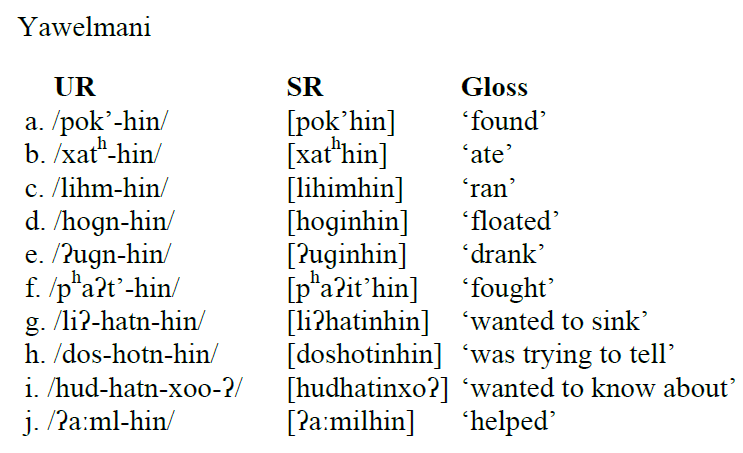
\includegraphics{../images/yawelmani.png}
\end{figure}

\newpage

{\large Question 2}\\

Source: Final Exam Dataset\\

Explain what the underlying representation of these morphemes would be and why.\\

`dig', `future'

\begin{figure}[H]
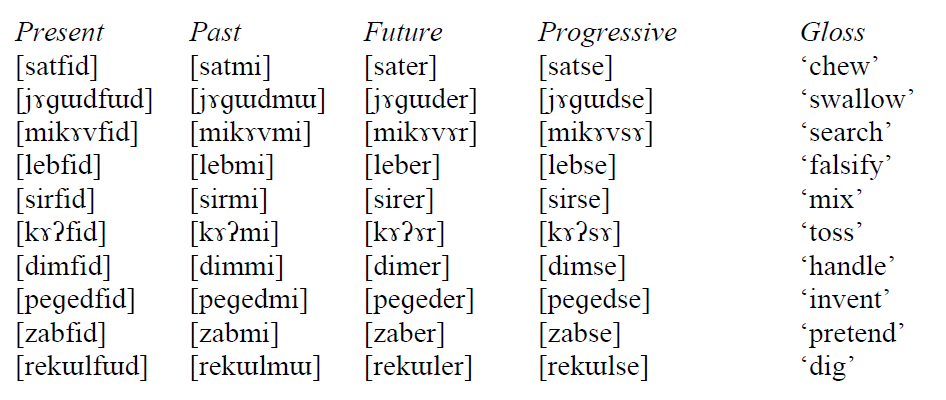
\includegraphics{../images/final_dataset.png}
\end{figure}

\newpage

{\large Question 3}\\

Source: Day 8 Handout, Question 3\\

Explain what you see in the spectrogram that tells you about the properties of the sounds in the pictured word.\\

\begin{figure}[H]
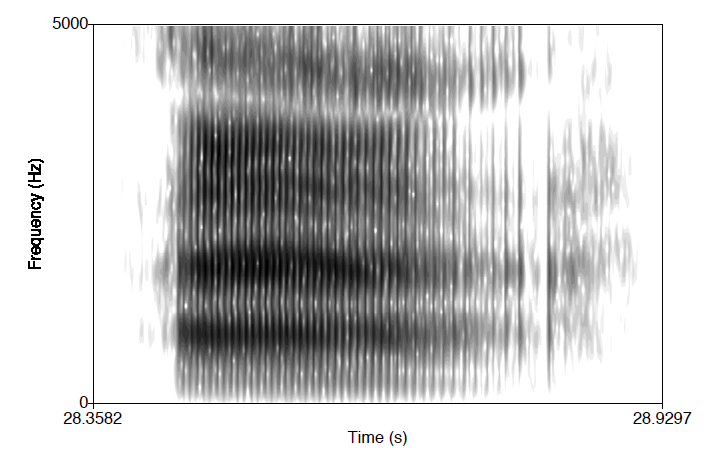
\includegraphics{../images/spectrogram_aaah.png}
\end{figure}

\newpage

{\large Question 4}\\

Source: Quiz 8, Question 6\\

Explain why this is an incorrect statement.\\

Nasal consonants are {[+continuant]} because they lack a central occlusion in the vocal tract.


\newpage

{\large Question 5}\\

Source: Day 12 Handout, Question 5\\

Explain which of the three rules will apply to the form given below, and whether each of those rules would have an effect or not.\\

Peng’s Tone-Mapping Procedure for Mende: \begin{enumerate} \item L-to-R association: Associate the first tone to the first TBU, the second tone to the second TBU, and so on, until all tones or all TBUS are exhausted. \item Last-TBU Linking: Associate any remaining unlinked tones to the last TBU. \item Last-Tone Linking: Associate the last tone to any TBU without a tone. \end{enumerate}

\begin{figure}[H]
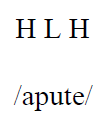
\includegraphics{../images/mendetone_a.png}
\end{figure}

\newpage

{\large Question 6}\\

Source: Day 9 Handout, Question 3\\

Explain which morpheme(s) in this dataset alternate and how that helps you do a phonological analysis.\\

\begin{figure}[H]
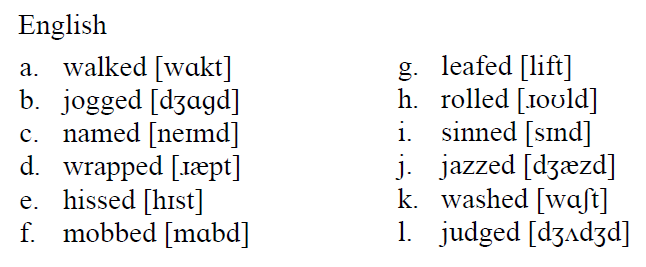
\includegraphics{../images/english_past.png}
\end{figure}

\newpage

\begin{center}
\textbf{{\color{red}{\HUGE END OF EXAM}}}\\

\end{center}
\newpage

\begin{center}
\textbf{{\color{blue}{\HUGE START OF EXAM\\}}}

\textbf{{\color{blue}{\HUGE Student ID: 7336\\}}}

\textbf{{\color{blue}{\HUGE 9:50 - 10:10 AM\\}}}

\end{center}
\newpage

{\large Question 1}\\

Source: Day 11 Handout, Question 12\\

Explain why what you’re analyzing in the following dataset either is or is not an alternation.\\

\begin{figure}[H]
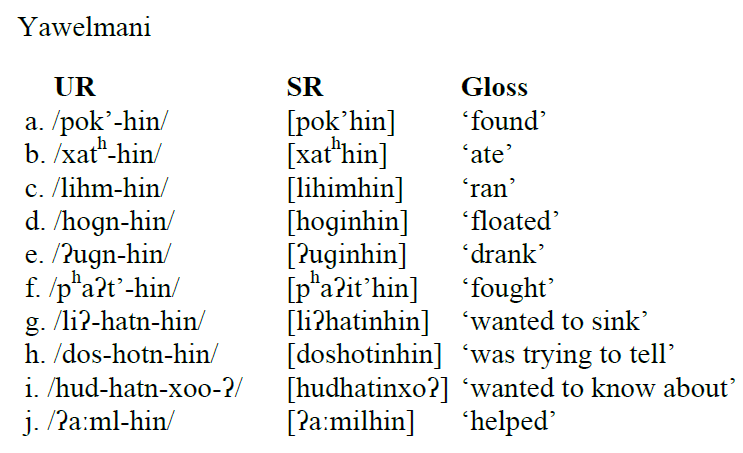
\includegraphics{../images/yawelmani.png}
\end{figure}

\newpage

{\large Question 2}\\

Source: Day 10 Discussion\\

Explain why the given feature's value varies across this set of sounds.\\

{[anterior]}

fricatives


\newpage

{\large Question 3}\\

Source: Final Exam Dataset\\

Explain what the underlying representation of these morphemes would be and why.\\

`dig', `future'

\begin{figure}[H]
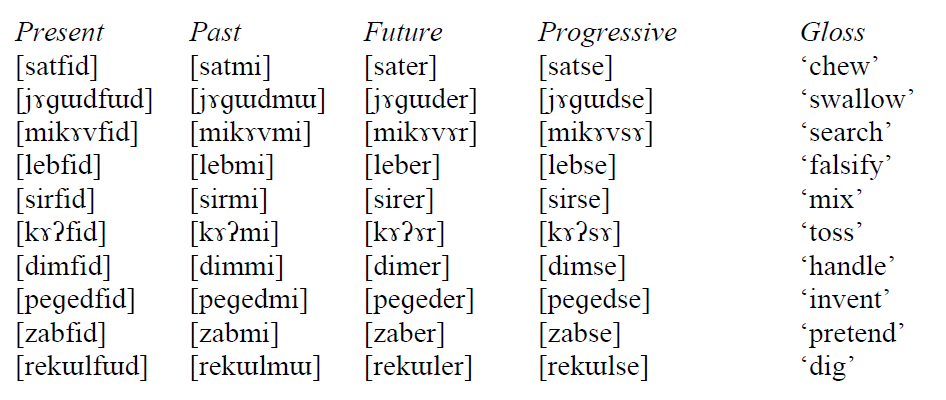
\includegraphics{../images/final_dataset.png}
\end{figure}

\newpage

{\large Question 4}\\

Source: Day 8 Handout, Question 4\\

Explain how each component of the description below gives you information about the sound being described.\\

This consonant is characterized by having a lot of random noise in the spectrogram, with no clear formant structure at all. It tends to be longer and louder than other similar consonants. There is no voice bar, and the majority of the noise created by this consonant is at relatively high frequencies.


\newpage

{\large Question 5}\\

Source: Quiz 10, Question 1\\

Section 4.2 of chapter 13 in the Peng textbook presented an autosegmental analysis of Mende tone distribution. Explain why the form shown below should NOT be the UR for any morpheme in Mende.\\

\begin{figure}[H]
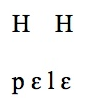
\includegraphics{../images/mende_house_b.png}
\end{figure}

\newpage

{\large Question 6}\\

Source: Day 11 Handout, Question 14\\

How does syllabification play a role in the analysis of the phonological relationship between tense and lax high vowels in Quebec French?\\

\begin{figure}[H]
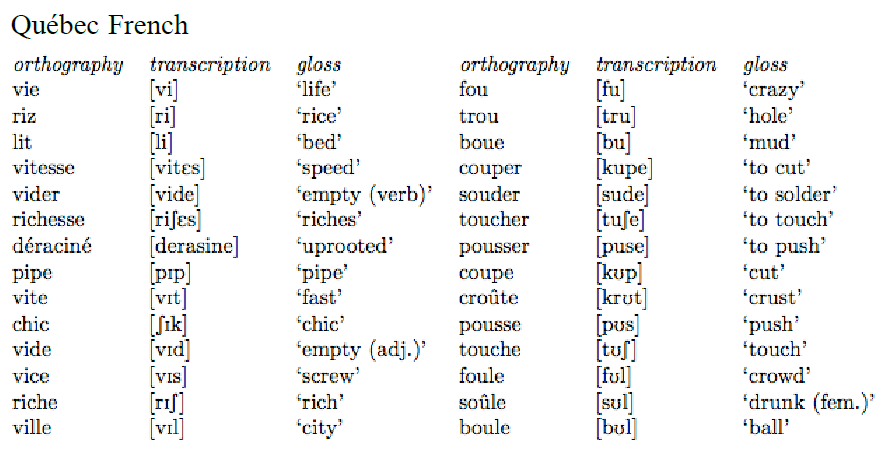
\includegraphics{../images/quebecfrench.png}
\end{figure}

\newpage

\begin{center}
\textbf{{\color{red}{\HUGE END OF EXAM}}}\\

\end{center}
\newpage

\begin{center}
\textbf{{\color{blue}{\HUGE START OF EXAM\\}}}

\textbf{{\color{blue}{\HUGE Student ID: 3514\\}}}

\textbf{{\color{blue}{\HUGE 10:10 - 10:30 AM\\}}}

\end{center}
\newpage

{\large Question 1}\\

Source: Day 8 Handout, Question 1\\

Explain what (if anything) the letter below represents on this waveform.\\

E

\begin{figure}[H]
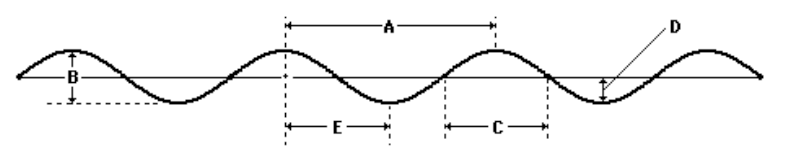
\includegraphics{../images/sinusoid.png}
\end{figure}

\newpage

{\large Question 2}\\

Source: Final Exam Dataset\\

Explain what the underlying representation of these morphemes would be and why.\\

`invent', `progressive'

\begin{figure}[H]
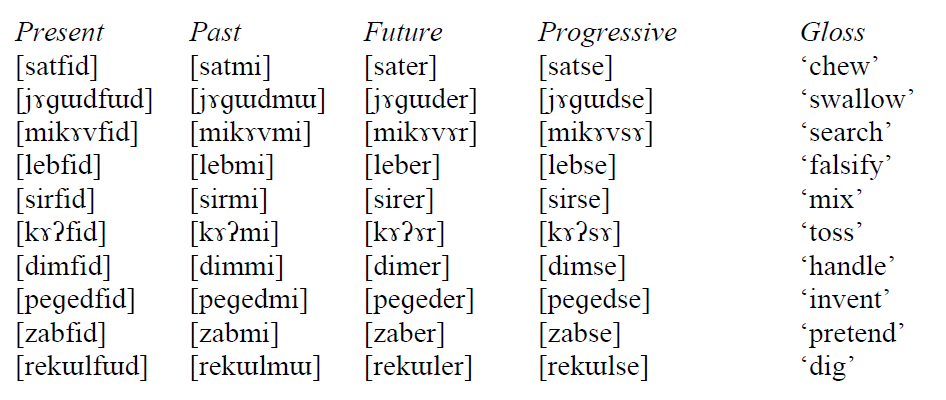
\includegraphics{../images/final_dataset.png}
\end{figure}

\newpage

{\large Question 3}\\

Source: Day 11 Handout, Question 16\\

How does syllabification play a role in the analysis of Tibetan numerals?\\

\begin{figure}[H]
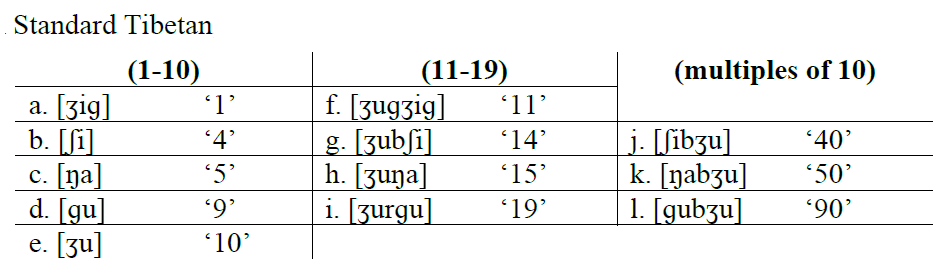
\includegraphics{../images/tibetan.png}
\end{figure}

\newpage

{\large Question 4}\\

Source: Day 12 Handout, Question 5\\

Explain which of the three rules will apply to the form given below, and whether each of those rules would have an effect or not.\\

Peng’s Tone-Mapping Procedure for Mende: \begin{enumerate} \item L-to-R association: Associate the first tone to the first TBU, the second tone to the second TBU, and so on, until all tones or all TBUS are exhausted. \item Last-TBU Linking: Associate any remaining unlinked tones to the last TBU. \item Last-Tone Linking: Associate the last tone to any TBU without a tone. \end{enumerate}

\begin{figure}[H]
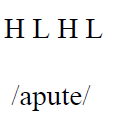
\includegraphics{../images/mendetone_d.png}
\end{figure}

\newpage

{\large Question 5}\\

Source: Day 10 Discussion\\

Explain why the given feature's value varies across this set of sounds.\\

{[voice]}

glottalized obstruents


\newpage

{\large Question 6}\\

Source: Day 9 Handout, Question 5\\

Explain which morpheme(s) in this dataset alternate and how that helps you do a phonological analysis.\\

\begin{figure}[H]
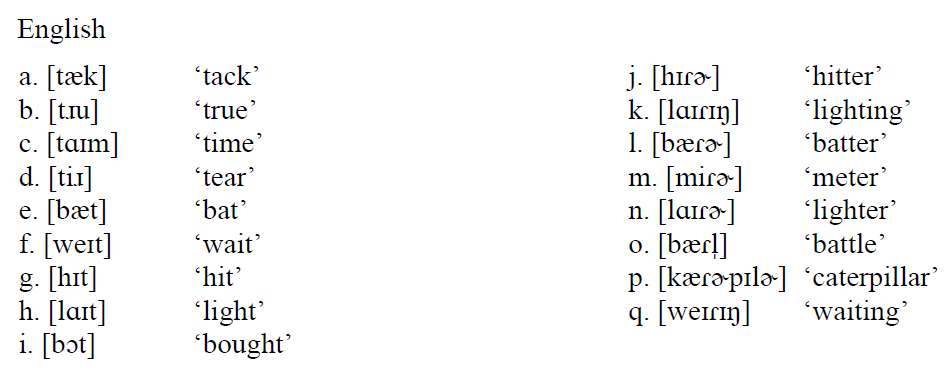
\includegraphics{../images/english_t_flap.png}
\end{figure}

\newpage

\begin{center}
\textbf{{\color{red}{\HUGE END OF EXAM}}}\\

\end{center}
\newpage

\begin{center}
\textbf{{\color{blue}{\HUGE START OF EXAM\\}}}

\textbf{{\color{blue}{\HUGE Student ID: 3129\\}}}

\textbf{{\color{blue}{\HUGE 10:30 - 10:50 AM\\}}}

\end{center}
\newpage

{\large Question 1}\\

Source: Quiz 10, Question 3\\

Section 4.2 of chapter 13 in the Peng textbook presented an autosegmental analysis of Mende tone distribution. Explain why the form shown below should NOT be the UR for any morpheme in Mende.\\

\begin{figure}[H]
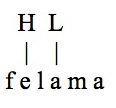
\includegraphics{../images/mende_junction_a.png}
\end{figure}

\newpage

{\large Question 2}\\

Source: Day 11 Handout, Question 15\\

Do these two signs have the same syllable structure or different, and why?\\

\begin{figure}[H]
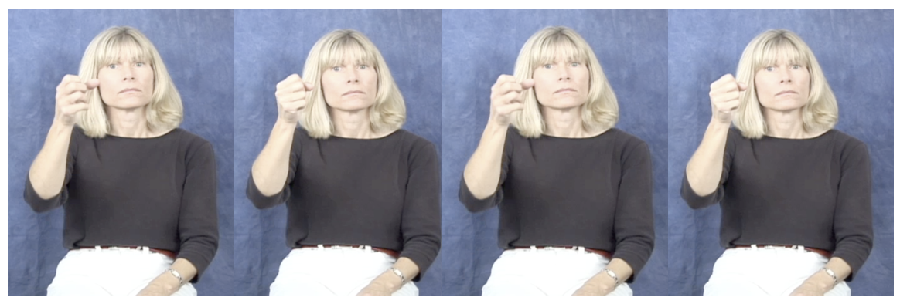
\includegraphics{../images/asl_milk.png}
\caption{MILK}
\end{figure}
\begin{figure}[H]
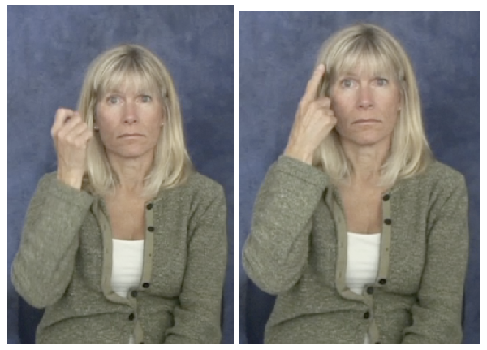
\includegraphics{../images/asl_understand.png}
\caption{UNDERSTAND}
\end{figure}

\newpage

{\large Question 3}\\

Source: Final Exam Dataset\\

Explain what the basic phonological analysis of this dataset is, and what the key pieces of evidence are.\\

\begin{figure}[H]
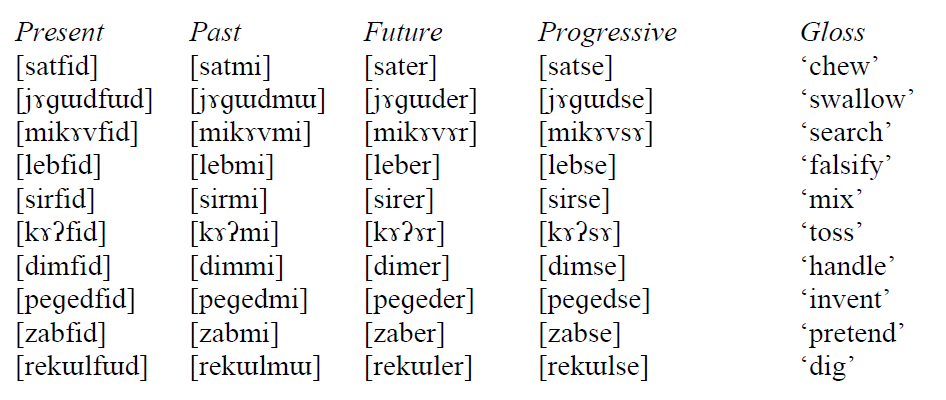
\includegraphics{../images/final_dataset.png}
\end{figure}

\newpage

{\large Question 4}\\

Source: Day 8 Discussion\\

Briefly explain source-filter theory.\\


\newpage

{\large Question 5}\\

Source: Quiz 8, Question 3\\

Explain why this featural specification either does or does not match the given sound.\\

{[-consonantal]}, {[-sonorant]}

{[u]}


\newpage

{\large Question 6}\\

Source: Day 9 Handout, Question 4\\

Explain which morpheme(s) in this dataset alternate and how that helps you do a phonological analysis.\\

\begin{figure}[H]
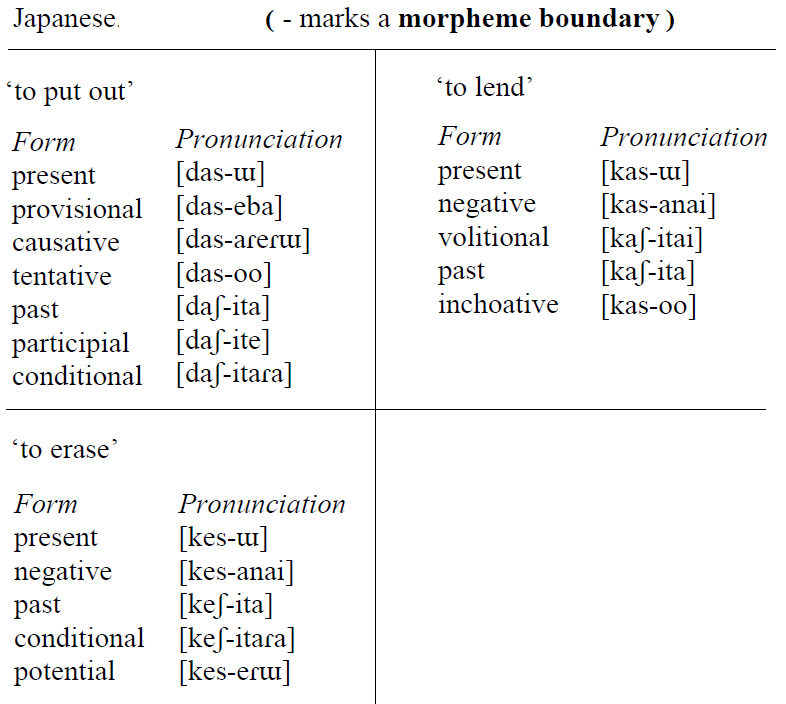
\includegraphics{../images/japanese_verbs.png}
\end{figure}

\newpage

\begin{center}
\textbf{{\color{red}{\HUGE END OF EXAM}}}\\

\end{center}
\newpage

\begin{center}
\textbf{{\color{blue}{\HUGE START OF EXAM\\}}}

\textbf{{\color{blue}{\HUGE Student ID: 3288\\}}}

\textbf{{\color{blue}{\HUGE 10:50 - 11:10 AM\\}}}

\end{center}
\newpage

{\large Question 1}\\

Source: Day 9 Handout, Question 2\\

Explain why the concept of an alternation either is or is not useful for understanding this dataset.\\

\begin{figure}[H]
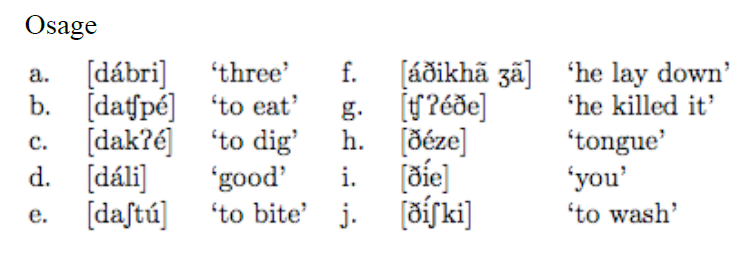
\includegraphics{../images/osage.png}
\end{figure}

\newpage

{\large Question 2}\\

Source: Day 10 Discussion\\

Explain why the given feature's value varies across this set of sounds.\\

{[sonorant]}

alveolars


\newpage

{\large Question 3}\\

Source: Final Exam Dataset\\

Explain what the underlying representation of these morphemes would be and why.\\

`mix', `past'

\begin{figure}[H]
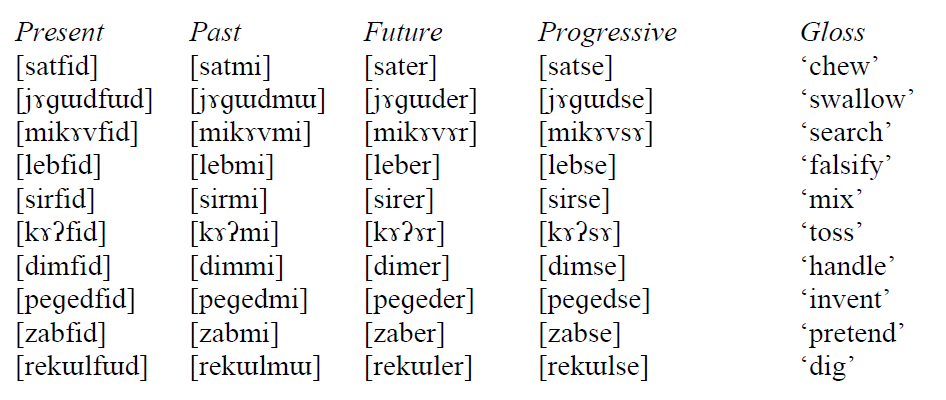
\includegraphics{../images/final_dataset.png}
\end{figure}

\newpage

{\large Question 4}\\

Source: Day 12 Handout, Question 5\\

Explain which of the three rules will apply to the form given below, and whether each of those rules would have an effect or not.\\

Peng’s Tone-Mapping Procedure for Mende: \begin{enumerate} \item L-to-R association: Associate the first tone to the first TBU, the second tone to the second TBU, and so on, until all tones or all TBUS are exhausted. \item Last-TBU Linking: Associate any remaining unlinked tones to the last TBU. \item Last-Tone Linking: Associate the last tone to any TBU without a tone. \end{enumerate}

\begin{figure}[H]
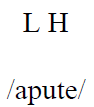
\includegraphics{../images/mendetone_c.png}
\end{figure}

\newpage

{\large Question 5}\\

Source: Day 11 Handout, Question 5\\

Explain why this template either does or does not allow syllables of this type to occur.\\

CCV

\begin{figure}[H]
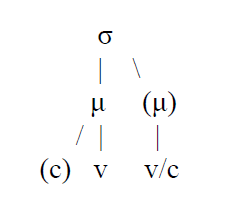
\includegraphics{../images/ponapean_syllabletemplate.png}
\end{figure}

\newpage

{\large Question 6}\\

Source: Day 8 Handout, Question 3\\

Explain what you see in the spectrogram that tells you about the properties of the sounds in the pictured word.\\

\begin{figure}[H]
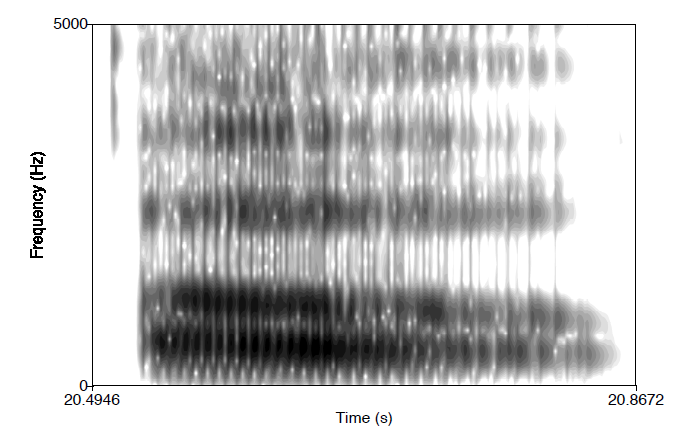
\includegraphics{../images/spectrogram_oh.png}
\end{figure}

\newpage

\begin{center}
\textbf{{\color{red}{\HUGE END OF EXAM}}}\\

\end{center}
\newpage

\begin{center}
\textbf{{\color{blue}{\HUGE START OF EXAM\\}}}

\textbf{{\color{blue}{\HUGE Student ID: 9450\\}}}

\textbf{{\color{blue}{\HUGE 11:10 - 11:30 AM\\}}}

\end{center}
\newpage

{\large Question 1}\\

Source: Day 11 Handout, Question 5\\

Explain why this template either does or does not allow syllables of this type to occur.\\

VCC

\begin{figure}[H]
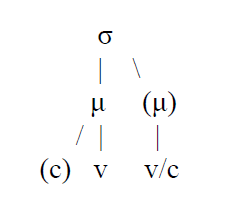
\includegraphics{../images/ponapean_syllabletemplate.png}
\end{figure}

\newpage

{\large Question 2}\\

Source: Quiz 8, Question 6\\

Explain why this is an incorrect statement.\\

Nasal consonants are {[+continuant]}, because you can continue to make the sound for a long period of time (until you run out of breath).


\newpage

{\large Question 3}\\

Source: Final Exam Dataset\\

Explain what the underlying representation of these morphemes would be and why.\\

`dig', `future'

\begin{figure}[H]
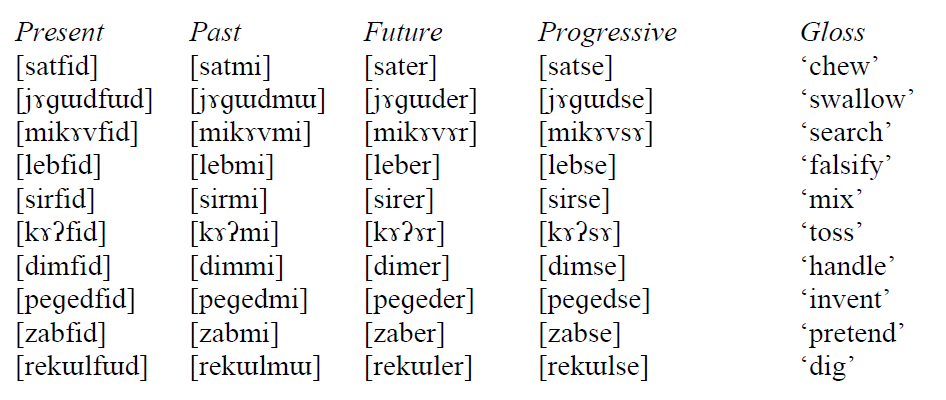
\includegraphics{../images/final_dataset.png}
\end{figure}

\newpage

{\large Question 4}\\

Source: Quiz 7, Question 8\\

Based on this data from Lamba, explain why the pair given below either does or does not show that the consonants preceding the morpheme for `with' are NOT responsible for the variation between [-il] and [-el].\\

čit-a \& čit-il-a

\begin{figure}[H]
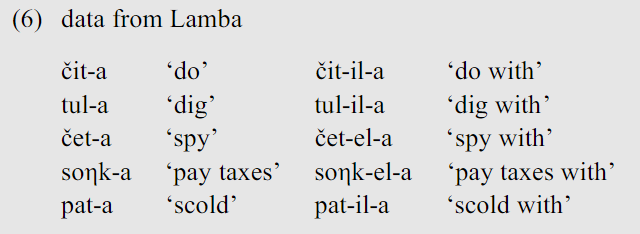
\includegraphics{../images/peng119_lamba.png}
\end{figure}

\newpage

{\large Question 5}\\

Source: Day 8 Handout, Question 3\\

Explain what you see in the spectrogram that tells you about the properties of the sounds in the pictured word.\\

\begin{figure}[H]
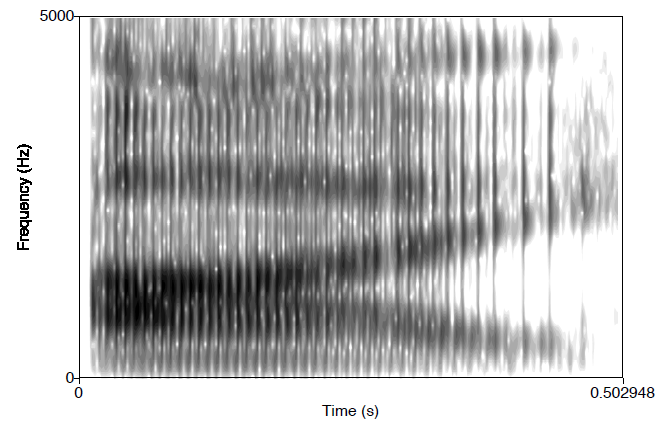
\includegraphics{../images/spectrogram_I.png}
\end{figure}

\newpage

{\large Question 6}\\

Source: Day 12 Handout, Question 5\\

Explain which of the three rules will apply to the form given below, and whether each of those rules would have an effect or not.\\

Peng’s Tone-Mapping Procedure for Mende: \begin{enumerate} \item L-to-R association: Associate the first tone to the first TBU, the second tone to the second TBU, and so on, until all tones or all TBUS are exhausted. \item Last-TBU Linking: Associate any remaining unlinked tones to the last TBU. \item Last-Tone Linking: Associate the last tone to any TBU without a tone. \end{enumerate}

\begin{figure}[H]
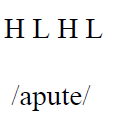
\includegraphics{../images/mendetone_d.png}
\end{figure}

\newpage

\begin{center}
\textbf{{\color{red}{\HUGE END OF EXAM}}}\\

\end{center}
\newpage

\begin{center}
\textbf{{\color{blue}{\HUGE START OF EXAM\\}}}

\textbf{{\color{blue}{\HUGE Student ID: 2357\\}}}

\textbf{{\color{blue}{\HUGE 11:30 - 11:50 AM\\}}}

\end{center}
\newpage

{\large Question 1}\\

Source: Quiz 10, Question 3\\

Section 4.2 of chapter 13 in the Peng textbook presented an autosegmental analysis of Mende tone distribution. Explain why the form shown below should NOT be the UR for any morpheme in Mende.\\

\begin{figure}[H]
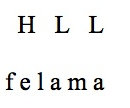
\includegraphics{../images/mende_junction_b.png}
\end{figure}

\newpage

{\large Question 2}\\

Source: Final Exam Dataset\\

Explain what the underlying representation of these morphemes would be and why.\\

`dig', `future'

\begin{figure}[H]
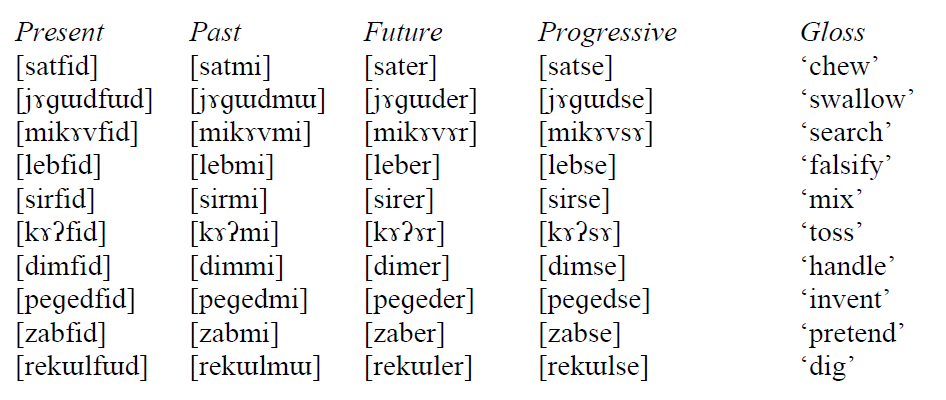
\includegraphics{../images/final_dataset.png}
\end{figure}

\newpage

{\large Question 3}\\

Source: Day 11 Handout, Question 6\\

Explain why this structure either is or is not a correct application of the rule-based approach to syllabification, assuming that both the onset rule and the coda rule apply in this language, and the onset rule comes before the coda rule.\\

\begin{figure}[H]
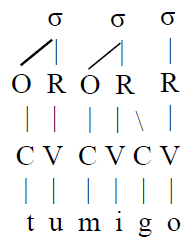
\includegraphics{../images/pengrules_tumigo_no.png}
\end{figure}
\begin{figure}[H]
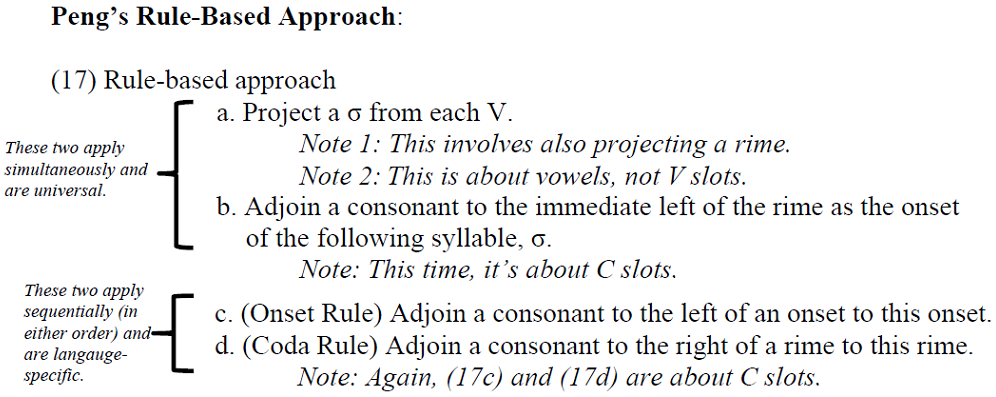
\includegraphics{../images/peng_rules.png}
\end{figure}

\newpage

{\large Question 4}\\

Source: Day 8 Handout, Question 1\\

Explain what (if anything) the letter below represents on this waveform.\\

D

\begin{figure}[H]
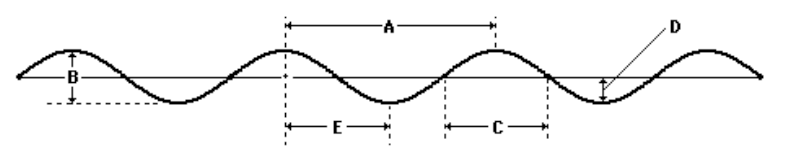
\includegraphics{../images/sinusoid.png}
\end{figure}

\newpage

{\large Question 5}\\

Source: Day 10 Handout, Question 6 (Day 7 Handout, Question 10)\\

Explain how you should use phonological features in this rule. Which parts of the rule should include features, and what features might they be? You don't have to give an exact set of features, but what kinds of features would be involved?\\

/ð/ → {[d]} / \_\_ {[a]}

\begin{figure}[H]
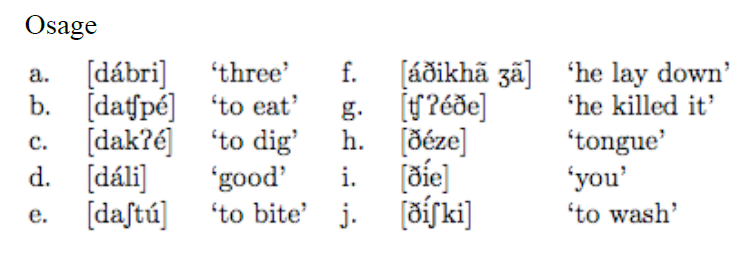
\includegraphics{../images/osage.png}
\end{figure}

\newpage

{\large Question 6}\\

Source: Quiz 7, Question 8\\

Based on this data from Lamba, explain why the pair given below either does or does not show that the consonants preceding the morpheme for `with' are NOT responsible for the variation between [-il] and [-el].\\

tul-il-a \& soŋk-el-a

\begin{figure}[H]
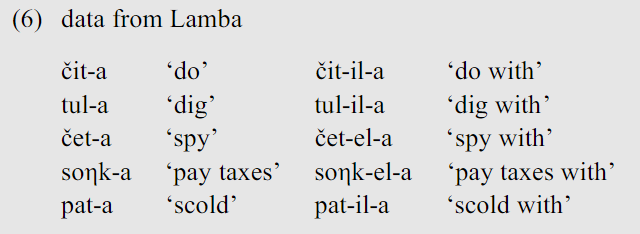
\includegraphics{../images/peng119_lamba.png}
\end{figure}

\newpage

\begin{center}
\textbf{{\color{red}{\HUGE END OF EXAM}}}\\

\end{center}
\newpage

\begin{center}
\textbf{{\color{blue}{\HUGE START OF EXAM\\}}}

\textbf{{\color{blue}{\HUGE Student ID: 1715\\}}}

\textbf{{\color{blue}{\HUGE 11:50 AM - 12:10 PM\\}}}

\end{center}
\newpage

{\large Question 1}\\

Source: Day 9 Handout, Question 1\\

Explain why the concept of an alternation either is or is not useful for understanding this dataset.\\

\begin{figure}[H]
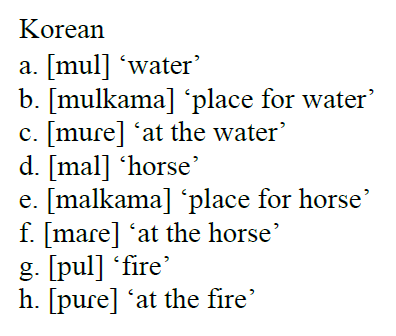
\includegraphics{../images/korean.png}
\end{figure}

\newpage

{\large Question 2}\\

Source: Final Exam Dataset\\

Explain what the underlying representation of these morphemes would be and why.\\

`mix', `past'

\begin{figure}[H]
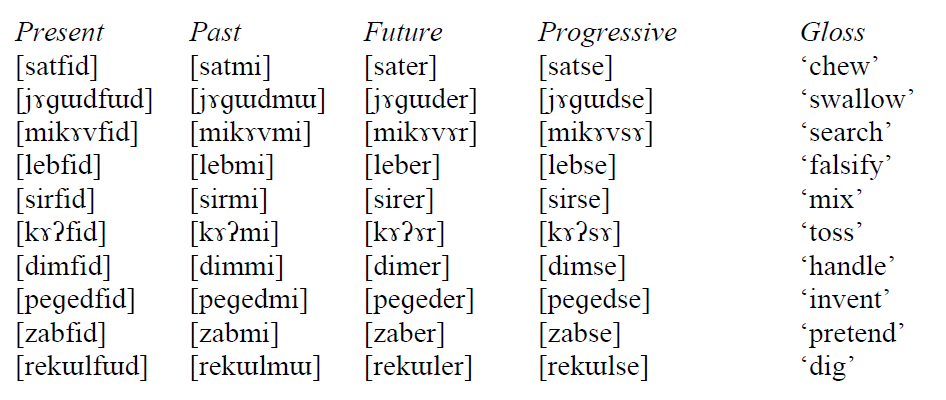
\includegraphics{../images/final_dataset.png}
\end{figure}

\newpage

{\large Question 3}\\

Source: Day 10 Discussion\\

Explain why the given feature's value varies across this set of sounds.\\

{[sonorant]}

alveolars


\newpage

{\large Question 4}\\

Source: Quiz 6, Question 2\\

Explain what you see in the spectrogram that tells you about the properties of the sounds in the pictured word.\\

\begin{figure}[H]
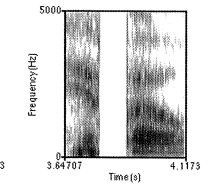
\includegraphics{../images/spectrogram_hippo.png}
\end{figure}

\newpage

{\large Question 5}\\

Source: Quiz 10, Question 1\\

Section 4.2 of chapter 13 in the Peng textbook presented an autosegmental analysis of Mende tone distribution. Explain why the form shown below should NOT be the UR for any morpheme in Mende.\\

\begin{figure}[H]
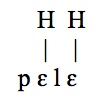
\includegraphics{../images/mende_house_e.png}
\end{figure}

\newpage

{\large Question 6}\\

Source: Day 11 Handout, Question 1\\

Explain how these examples help support the overall syllable structure of a syllable consisting of an onset and rime, and the rime consisting of a nucleus and coda.\\

\begin{figure}[H]
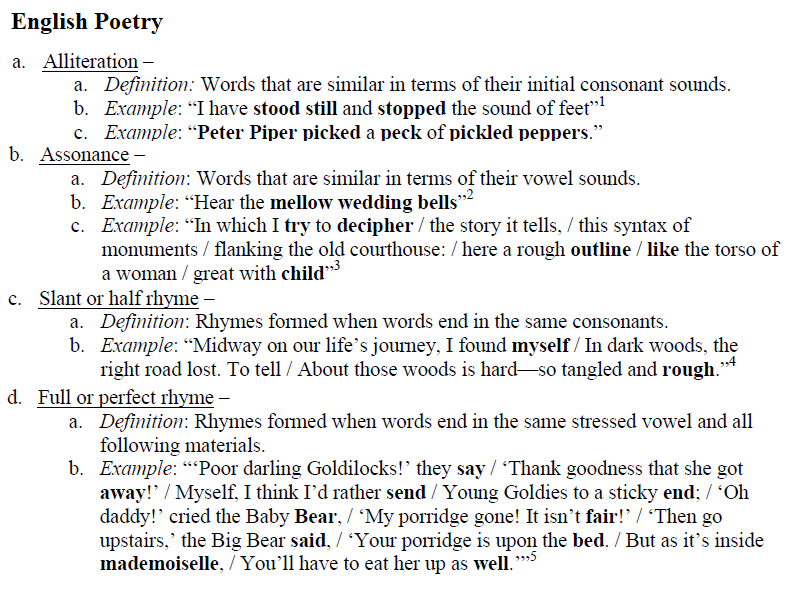
\includegraphics{../images/english_poetry.png}
\end{figure}

\newpage

\begin{center}
\textbf{{\color{red}{\HUGE END OF EXAM}}}\\

\end{center}
\newpage

\begin{center}
\textbf{{\color{blue}{\HUGE START OF EXAM\\}}}

\textbf{{\color{blue}{\HUGE Student ID: 2014\\}}}

\textbf{{\color{blue}{\HUGE 12:10 - 12:30 PM\\}}}

\end{center}
\newpage

{\large Question 1}\\

Source: Quiz 10, Question 3\\

Section 4.2 of chapter 13 in the Peng textbook presented an autosegmental analysis of Mende tone distribution. Explain why the form shown below should NOT be the UR for any morpheme in Mende.\\

\begin{figure}[H]
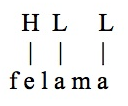
\includegraphics{../images/mende_junction_c.png}
\end{figure}

\newpage

{\large Question 2}\\

Source: Final Exam Dataset\\

Explain how you would go about figuring out what to analyse in this dataset.\\

\begin{figure}[H]
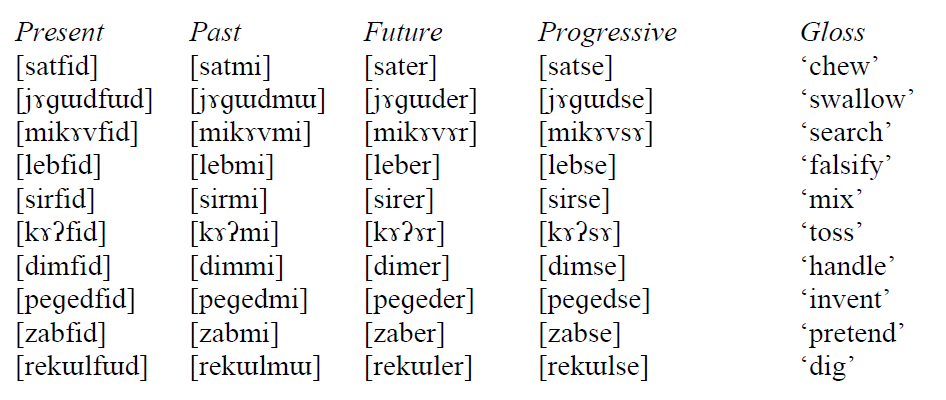
\includegraphics{../images/final_dataset.png}
\end{figure}

\newpage

{\large Question 3}\\

Source: Day 8 Handout, Question 3\\

Explain what you see in the spectrogram that tells you about the properties of the sounds in the pictured word.\\

\begin{figure}[H]
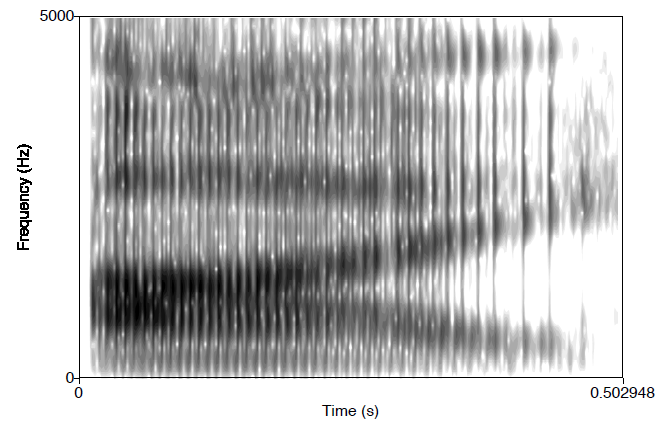
\includegraphics{../images/spectrogram_I.png}
\end{figure}

\newpage

{\large Question 4}\\

Source: Day 11 Handout, Question 5\\

Explain why this template either does or does not allow syllables of this type to occur.\\

CVVC

\begin{figure}[H]
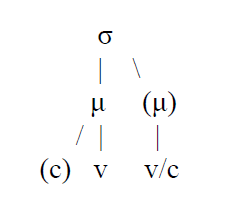
\includegraphics{../images/ponapean_syllabletemplate.png}
\end{figure}

\newpage

{\large Question 5}\\

Source: Quiz 7, Question 8\\

Based on this data from Lamba, explain why the pair given below either does or does not show that the consonants preceding the morpheme for `with' are NOT responsible for the variation between [-il] and [-el].\\

pat-il-a \& tul-il-a

\begin{figure}[H]
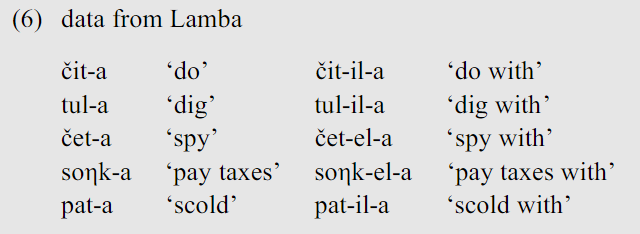
\includegraphics{../images/peng119_lamba.png}
\end{figure}

\newpage

{\large Question 6}\\

Source: Homework 5, Question 1\\

Explain which sound should be removed to make this a natural class, and what the minimum set of features would be to describe the resulting natural class.\\

{[i]}, {[ɪ]}, {[e]}, {[ɛ]}, {[æ]}, {[ɑ]}, {[ɔ]}, {[o]}, {[ʊ]}, {[u]}, {[ʒ]}, {[k]}, {[ɡ]}, {[ŋ]}, {[w]}


\newpage

\begin{center}
\textbf{{\color{red}{\HUGE END OF EXAM}}}\\

\end{center}
\newpage

\begin{center}
\textbf{{\color{blue}{\HUGE START OF EXAM\\}}}

\textbf{{\color{blue}{\HUGE Student ID: 4220\\}}}

\textbf{{\color{blue}{\HUGE 12:30 - 12:50 PM\\}}}

\end{center}
\newpage

{\large Question 1}\\

Source: Day 11 Handout, Question 12\\

Explain why what you’re analyzing in the following dataset either is or is not an alternation.\\

\begin{figure}[H]
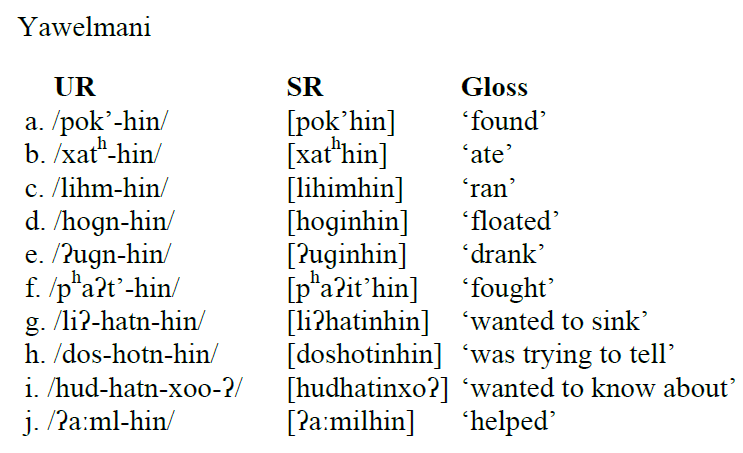
\includegraphics{../images/yawelmani.png}
\end{figure}

\newpage

{\large Question 2}\\

Source: Day 11 Handout, Question 8\\

Explain how you could modify the rule-based approach to take into account the sonority sequencing principle.\\

\begin{figure}[H]
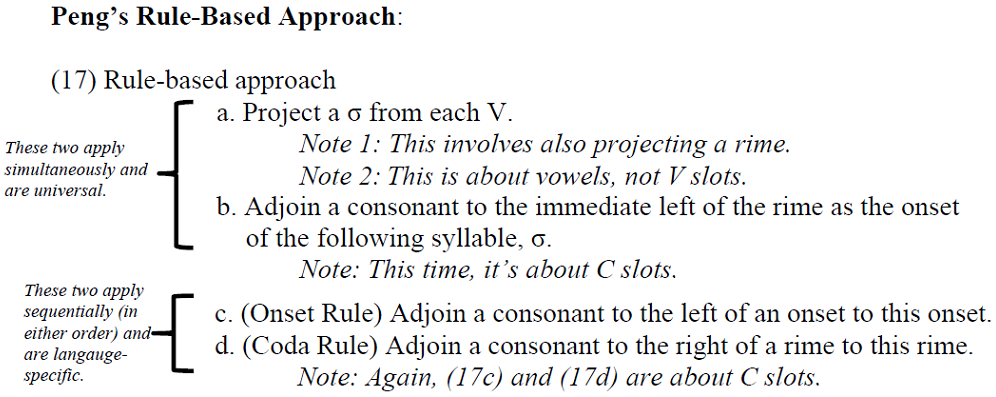
\includegraphics{../images/peng_rules.png}
\end{figure}

\newpage

{\large Question 3}\\

Source: Final Exam Dataset\\

Explain what the underlying representation of these morphemes would be and why.\\

`dig', `future'

\begin{figure}[H]
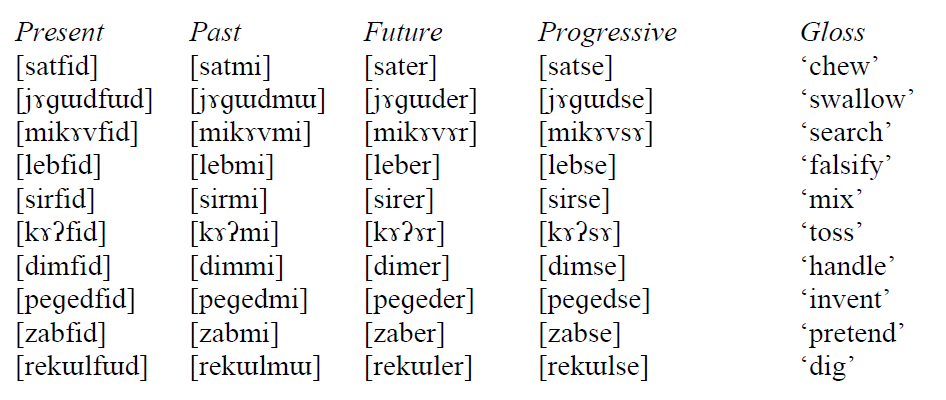
\includegraphics{../images/final_dataset.png}
\end{figure}

\newpage

{\large Question 4}\\

Source: Day 8 Handout, Question 7\\

Explain why each numbered, underlined statement is true or false. If it is false, explain one way that you could correct it.\\

$^{10}$\ul{Frequency is inversely related to pitch: high frequencies correspond to low pitches, and low frequencies correspond to high pitches.} Finally, there is the amplitude of the wave. $^{11}$\ul{The amplitude tells you how much pressure the molecules are under at any particular time.} $^{12}$\ul{The auditory correlate of amplitude is intensity}; this is a measure of perceived pressure.\\\\$^{13}$\ul{In speech, air is set in vibrating motion by the lungs, so the lungs} are the source of most speech sounds.


\newpage

{\large Question 5}\\

Source: Quiz 10, Question 1\\

Section 4.2 of chapter 13 in the Peng textbook presented an autosegmental analysis of Mende tone distribution. Explain why the form shown below should NOT be the UR for any morpheme in Mende.\\

\begin{figure}[H]
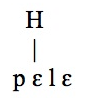
\includegraphics{../images/mende_house_a.png}
\end{figure}

\newpage

{\large Question 6}\\

Source: Day 10 Handout, Question 6 (Day 9 Handout, Question 5)\\

Explain how you should use phonological features in this rule. Which parts of the rule should include features, and what features might they be? You don't have to give an exact set of features, but what kinds of features would be involved?\\

/t/ → {[ɾ]} / \{{[vowel]},{[syllabic consonant]}\} \_\_ \{{[vowel]},{[syllabic consonant]}\}

\begin{figure}[H]
\includegraphics{../images/english_t_flap.png}
\end{figure}

\newpage

\begin{center}
\textbf{{\color{red}{\HUGE END OF EXAM}}}\\

\end{center}
\newpage

\begin{center}
\textbf{{\color{blue}{\HUGE START OF EXAM\\}}}

\textbf{{\color{blue}{\HUGE Student ID: 7661\\}}}

\textbf{{\color{blue}{\HUGE 12:50 - 1:10 PM\\}}}

\end{center}
\newpage

{\large Question 1}\\

Source: Day 8 Handout, Question 1\\

Explain what (if anything) the letter below represents on this waveform.\\

B

\begin{figure}[H]
\includegraphics{../images/sinusoid.png}
\end{figure}

\newpage

{\large Question 2}\\

Source: Final Exam Dataset\\

Give a good phonological description of the patterns in the dataset that should be analysed.\\

\begin{figure}[H]
\includegraphics{../images/final_dataset.png}
\end{figure}

\newpage

{\large Question 3}\\

Source: Day 12 Handout, Question 7\\

Explain how you would figure out the underlying representations of the suffix morphemes in this dataset.\\

\begin{figure}[H]
\includegraphics{../images/shona.png}
\end{figure}

\newpage

{\large Question 4}\\

Source: Day 11 Handout, Question 10\\

Explain why this structure either is or is not a correct application of the templatic-based approach to syllabification, using the provided template and assuming that syllabification proceeds from left to right.\\

\begin{figure}[H]
\includegraphics{../images/pengtemplate_uvkeman_no.png}
\end{figure}
\begin{figure}[H]
\includegraphics{../images/peng_template_withdiagram.png}
\end{figure}

\newpage

{\large Question 5}\\

Source: Quiz 8, Question 6\\

Explain why this is an incorrect statement.\\

Nasal consonants are {[-continuant]}, because they cannot be produced for an extended period of time.


\newpage

{\large Question 6}\\

Source: Quiz 7, Question 8\\

Based on this data from Lamba, explain why the pair given below either does or does not show that the consonants preceding the morpheme for `with' are NOT responsible for the variation between [-il] and [-el].\\

tul-il-a \& soŋk-el-a

\begin{figure}[H]
\includegraphics{../images/peng119_lamba.png}
\end{figure}

\newpage

\begin{center}
\textbf{{\color{red}{\HUGE END OF EXAM}}}\\

\end{center}
\newpage

\begin{center}
\textbf{{\color{blue}{\HUGE START OF EXAM\\}}}

\textbf{{\color{blue}{\HUGE Student ID: 8742\\}}}

\textbf{{\color{blue}{\HUGE 2:00 - 2:20 PM\\}}}

\end{center}
\newpage

{\large Question 1}\\

Source: Day 8 Handout, Question 1\\

Explain what (if anything) the letter below represents on this waveform.\\

C

\begin{figure}[H]
\includegraphics{../images/sinusoid.png}
\end{figure}

\newpage

{\large Question 2}\\

Source: Final Exam Dataset\\

Explain how you would go about figuring out what to analyse in this dataset.\\

\begin{figure}[H]
\includegraphics{../images/final_dataset.png}
\end{figure}

\newpage

{\large Question 3}\\

Source: Quiz 7, Question 8\\

Based on this data from Lamba, explain why the pair given below either does or does not show that the consonants preceding the morpheme for `with' are NOT responsible for the variation between [-il] and [-el].\\

čit-a \& čit-il-a

\begin{figure}[H]
\includegraphics{../images/peng119_lamba.png}
\end{figure}

\newpage

{\large Question 4}\\

Source: Day 11 Handout, Question 6\\

Explain why this structure either is or is not a correct application of the rule-based approach to syllabification, assuming that both the onset rule and the coda rule apply in this language, and the onset rule comes before the coda rule.\\

\begin{figure}[H]
\includegraphics{../images/pengrules_kaprosse_yes.png}
\end{figure}
\begin{figure}[H]
\includegraphics{../images/peng_rules.png}
\end{figure}

\newpage

{\large Question 5}\\

Source: Quiz 8, Question 3\\

Explain why this featural specification either does or does not match the given sound.\\

{[-consonantal]}, {[-sonorant]}

{[u]}


\newpage

{\large Question 6}\\

Source: Day 12 Handout, Question 7\\

What would be a good description of the alternation in this dataset?\\

\begin{figure}[H]
\includegraphics{../images/shona.png}
\end{figure}

\newpage

\begin{center}
\textbf{{\color{red}{\HUGE END OF EXAM}}}\\

\end{center}
\newpage

\begin{center}
\textbf{{\color{blue}{\HUGE START OF EXAM\\}}}

\textbf{{\color{blue}{\HUGE Student ID: 6948\\}}}

\textbf{{\color{blue}{\HUGE 2:20 - 2:40 PM\\}}}

\end{center}
\newpage

{\large Question 1}\\

Source: Day 11 Handout, Question 12\\

Explain why what you’re analyzing in the following dataset either is or is not an alternation.\\

\begin{figure}[H]
\includegraphics{../images/yawelmani.png}
\end{figure}

\newpage

{\large Question 2}\\

Source: Final Exam Dataset\\

Give a good phonological description of the patterns in the dataset that should be analysed.\\

\begin{figure}[H]
\includegraphics{../images/final_dataset.png}
\end{figure}

\newpage

{\large Question 3}\\

Source: Day 12 Handout, Question 6\\

Explain how you would figure out the tone-mapping procedures that apply in this dataset.\\

\begin{figure}[H]
\includegraphics{../images/kukuya.png}
\end{figure}

\newpage

{\large Question 4}\\

Source: Day 11 Discussion\\

Explain why the sonority sequencing principle would block the syllabification of [n] and [t] of [n.ta] into one syllable in Ponapean.\\


\newpage

{\large Question 5}\\

Source: Homework 5, Question 1\\

Explain which sound should be removed to make this a natural class, and what the minimum set of features would be to describe the resulting natural class.\\

{[i]}, {[ɪ]}, {[ɛ]}, {[u]}, {[ʊ]}


\newpage

{\large Question 6}\\

Source: Day 8 Handout, Question 6\\

Explain what you see in the spectrogram that tells you about the properties of the sounds in the pictured word.\\

\begin{figure}[H]
\includegraphics{../images/spectrogram_suit.png}
\end{figure}

\newpage

\begin{center}
\textbf{{\color{red}{\HUGE END OF EXAM}}}\\

\end{center}
\newpage

\begin{center}
\textbf{{\color{blue}{\HUGE START OF EXAM\\}}}

\textbf{{\color{blue}{\HUGE Student ID: 2931\\}}}

\textbf{{\color{blue}{\HUGE 2:40 - 3:00 PM\\}}}

\end{center}
\newpage

{\large Question 1}\\

Source: Day 11 Handout, Question 5\\

Explain why this template either does or does not allow syllables of this type to occur.\\

CVVC

\begin{figure}[H]
\includegraphics{../images/ponapean_syllabletemplate.png}
\end{figure}

\newpage

{\large Question 2}\\

Source: Final Exam Dataset\\

Explain what rule or rules would apply in this dataset and how you know.\\

\begin{figure}[H]
\includegraphics{../images/final_dataset.png}
\end{figure}

\newpage

{\large Question 3}\\

Source: Day 10 Discussion\\

Explain why phonological features are used instead of phonetic characteristics in analyzing datasets.\\


\newpage

{\large Question 4}\\

Source: Day 12 Handout, Question 5\\

Explain which of the three rules will apply to the form given below, and whether each of those rules would have an effect or not.\\

Peng’s Tone-Mapping Procedure for Mende: \begin{enumerate} \item L-to-R association: Associate the first tone to the first TBU, the second tone to the second TBU, and so on, until all tones or all TBUS are exhausted. \item Last-TBU Linking: Associate any remaining unlinked tones to the last TBU. \item Last-Tone Linking: Associate the last tone to any TBU without a tone. \end{enumerate}

\begin{figure}[H]
\includegraphics{../images/mendetone_a.png}
\end{figure}

\newpage

{\large Question 5}\\

Source: Quiz 7, Question 8\\

Based on this data from Lamba, explain why the pair given below either does or does not show that the consonants preceding the morpheme for `with' are NOT responsible for the variation between [-il] and [-el].\\

čet-el-a \& čit-il-a

\begin{figure}[H]
\includegraphics{../images/peng119_lamba.png}
\end{figure}

\newpage

{\large Question 6}\\

Source: Day 8 Handout, Question 1\\

Explain what (if anything) the letter below represents on this waveform.\\

D

\begin{figure}[H]
\includegraphics{../images/sinusoid.png}
\end{figure}

\newpage

\begin{center}
\textbf{{\color{red}{\HUGE END OF EXAM}}}\\

\end{center}
\newpage

\begin{center}
\textbf{{\color{blue}{\HUGE START OF EXAM\\}}}

\textbf{{\color{blue}{\HUGE Student ID: 6801\\}}}

\textbf{{\color{blue}{\HUGE 3:00 - 3:20 PM\\}}}

\end{center}
\newpage

{\large Question 1}\\

Source: Quiz 10, Question 1\\

Section 4.2 of chapter 13 in the Peng textbook presented an autosegmental analysis of Mende tone distribution. Explain why the form shown below should NOT be the UR for any morpheme in Mende.\\

\begin{figure}[H]
\includegraphics{../images/mende_house_b.png}
\end{figure}

\newpage

{\large Question 2}\\

Source: Final Exam Dataset\\

Explain what the underlying representation of these morphemes would be and why.\\

`dig', `future'

\begin{figure}[H]
\includegraphics{../images/final_dataset.png}
\end{figure}

\newpage

{\large Question 3}\\

Source: Quiz 7, Question 8\\

Based on this data from Lamba, explain why the pair given below either does or does not show that the consonants preceding the morpheme for `with' are NOT responsible for the variation between [-il] and [-el].\\

čet-el-a \& čit-il-a

\begin{figure}[H]
\includegraphics{../images/peng119_lamba.png}
\end{figure}

\newpage

{\large Question 4}\\

Source: Day 11 Handout, Question 10\\

Explain why this structure either is or is not a correct application of the templatic-based approach to syllabification, using the provided template and assuming that syllabification proceeds from left to right.\\

\begin{figure}[H]
\includegraphics{../images/pengtemplate_fletoldu_no.png}
\end{figure}
\begin{figure}[H]
\includegraphics{../images/peng_template_withdiagram.png}
\end{figure}

\newpage

{\large Question 5}\\

Source: Quiz 8, Question 3\\

Explain why this featural specification either does or does not match the given sound.\\

{[+consonantal]}, {[+sonorant]}

{[m]}


\newpage

{\large Question 6}\\

Source: Day 8 Handout, Question 3\\

Explain what you see in the spectrogram that tells you about the properties of the sounds in the pictured word.\\

\begin{figure}[H]
\includegraphics{../images/spectrogram_oh.png}
\end{figure}

\newpage

\begin{center}
\textbf{{\color{red}{\HUGE END OF EXAM}}}\\

\end{center}
\newpage

\begin{center}
\textbf{{\color{blue}{\HUGE START OF EXAM\\}}}

\textbf{{\color{blue}{\HUGE Student ID: 1743\\}}}

\textbf{{\color{blue}{\HUGE 3:20 - 3:40 PM\\}}}

\end{center}
\newpage

{\large Question 1}\\

Source: Day 9 Handout, Question 1\\

Explain why the concept of an alternation either is or is not useful for understanding this dataset.\\

\begin{figure}[H]
\includegraphics{../images/korean.png}
\end{figure}

\newpage

{\large Question 2}\\

Source: Final Exam Dataset\\

Explain what the underlying representation of these morphemes would be and why.\\

`dig', `future'

\begin{figure}[H]
\includegraphics{../images/final_dataset.png}
\end{figure}

\newpage

{\large Question 3}\\

Source: Quiz 8, Question 6\\

Explain why this is an incorrect statement.\\

Nasal consonants are {[+continuant]} because they lack a central occlusion in the vocal tract.


\newpage

{\large Question 4}\\

Source: Day 12 Handout, Question 5\\

Explain which of the three rules will apply to the form given below, and whether each of those rules would have an effect or not.\\

Peng’s Tone-Mapping Procedure for Mende: \begin{enumerate} \item L-to-R association: Associate the first tone to the first TBU, the second tone to the second TBU, and so on, until all tones or all TBUS are exhausted. \item Last-TBU Linking: Associate any remaining unlinked tones to the last TBU. \item Last-Tone Linking: Associate the last tone to any TBU without a tone. \end{enumerate}

\begin{figure}[H]
\includegraphics{../images/mendetone_b.png}
\end{figure}

\newpage

{\large Question 5}\\

Source: Day 11 Handout, Question 6\\

Explain why this structure either is or is not a correct application of the rule-based approach to syllabification, assuming that both the onset rule and the coda rule apply in this language, and the onset rule comes before the coda rule.\\

\begin{figure}[H]
\includegraphics{../images/pengrules_kaprose_no.png}
\end{figure}
\begin{figure}[H]
\includegraphics{../images/peng_rules.png}
\end{figure}

\newpage

{\large Question 6}\\

Source: Quiz 6, Question 2\\

Explain what you see in the spectrogram that tells you about the properties of the sounds in the pictured word.\\

\begin{figure}[H]
\includegraphics{../images/spectrogram_hippo.png}
\end{figure}

\newpage

\begin{center}
\textbf{{\color{red}{\HUGE END OF EXAM}}}\\

\end{center}
\newpage

\begin{center}
\textbf{{\color{blue}{\HUGE START OF EXAM\\}}}

\textbf{{\color{blue}{\HUGE Student ID: 5581\\}}}

\textbf{{\color{blue}{\HUGE 3:40 - 4:00 PM\\}}}

\end{center}
\newpage

{\large Question 1}\\

Source: Quiz 10, Question 1\\

Section 4.2 of chapter 13 in the Peng textbook presented an autosegmental analysis of Mende tone distribution. Explain why the form shown below should NOT be the UR for any morpheme in Mende.\\

\begin{figure}[H]
\includegraphics{../images/mende_house_b.png}
\end{figure}

\newpage

{\large Question 2}\\

Source: Quiz 7, Question 8\\

Based on this data from Lamba, explain why the pair given below either does or does not show that the consonants preceding the morpheme for `with' are NOT responsible for the variation between [-il] and [-el].\\

pat-il-a \& tul-il-a

\begin{figure}[H]
\includegraphics{../images/peng119_lamba.png}
\end{figure}

\newpage

{\large Question 3}\\

Source: Final Exam Dataset\\

Give a good phonological description of the patterns in the dataset that should be analysed.\\

\begin{figure}[H]
\includegraphics{../images/final_dataset.png}
\end{figure}

\newpage

{\large Question 4}\\

Source: Day 11 Handout, Question 12\\

Explain how understanding syllable structure helps understand the motivation for the process(es) seen in this data.\\

\begin{figure}[H]
\includegraphics{../images/yawelmani.png}
\end{figure}

\newpage

{\large Question 5}\\

Source: Day 8 Handout, Question 4\\

Explain how each component of the description below gives you information about the sound being described.\\

This consonant is characterized by having the adjacent second and third formants ``pinched'' together; that is, F3 moves down and F2 moves up if you go from a vowel into this consonant. There is often a clear voice bar, but there’s no evidence of formants in the consonant itself. In fact, there’s not much energy during the consonant at all.


\newpage

{\large Question 6}\\

Source: Day 10 Handout, Question 6 (Day 7 Handout, Question 8)\\

Explain how you should use phonological features in this rule. Which parts of the rule should include features, and which features should be used?\\

/ʊ/ → {[ɯ]} / {[unrounded vowel]} C$_0$ \_\_

\begin{figure}[H]
\includegraphics{../images/tamil.png}
\end{figure}

\newpage

\begin{center}
\textbf{{\color{red}{\HUGE END OF EXAM}}}\\

\end{center}
\newpage

\begin{center}
\textbf{{\color{blue}{\HUGE START OF EXAM\\}}}

\textbf{{\color{blue}{\HUGE Student ID: 2358\\}}}

\textbf{{\color{blue}{\HUGE 4:00 - 4:20 PM\\}}}

\end{center}
\newpage

{\large Question 1}\\

Source: Day 9 Handout, Question 2\\

Explain why the concept of an alternation either is or is not useful for understanding this dataset.\\

\begin{figure}[H]
\includegraphics{../images/osage.png}
\end{figure}

\newpage

{\large Question 2}\\

Source: Final Exam Dataset\\

Explain what the underlying representation of these morphemes would be and why.\\

`mix', `past'

\begin{figure}[H]
\includegraphics{../images/final_dataset.png}
\end{figure}

\newpage

{\large Question 3}\\

Source: Day 8 Handout, Question 3\\

Explain what you see in the spectrogram that tells you about the properties of the sounds in the pictured word.\\

\begin{figure}[H]
\includegraphics{../images/spectrogram_we.png}
\end{figure}

\newpage

{\large Question 4}\\

Source: Day 12 Handout, Question 5\\

Explain which of the three rules will apply to the form given below, and whether each of those rules would have an effect or not.\\

Peng’s Tone-Mapping Procedure for Mende: \begin{enumerate} \item L-to-R association: Associate the first tone to the first TBU, the second tone to the second TBU, and so on, until all tones or all TBUS are exhausted. \item Last-TBU Linking: Associate any remaining unlinked tones to the last TBU. \item Last-Tone Linking: Associate the last tone to any TBU without a tone. \end{enumerate}

\begin{figure}[H]
\includegraphics{../images/mendetone_d.png}
\end{figure}

\newpage

{\large Question 5}\\

Source: Day 11 Handout, Question 8\\

Explain how you could modify the rule-based approach to take into account the sonority sequencing principle.\\

\begin{figure}[H]
\includegraphics{../images/peng_rules.png}
\end{figure}

\newpage

{\large Question 6}\\

Source: Day 10 Handout, Question 5\\

Explain why you either should or should not use phonological features in the CONTEXT of the given rule.\\

Vowel laxing: /i/ → {[ɪ]} / \{{[ɛ]}, {[ɔ]}\} C$_0$\_\_


\newpage

\begin{center}
\textbf{{\color{red}{\HUGE END OF EXAM}}}\\

\end{center}
\newpage

\begin{center}
\textbf{{\color{blue}{\HUGE START OF EXAM\\}}}

\textbf{{\color{blue}{\HUGE Student ID: 9918\\}}}

\textbf{{\color{blue}{\HUGE 4:20 - 4:40 PM\\}}}

\end{center}
\newpage

{\large Question 1}\\

Source: Day 9 Handout, Question 1\\

Explain why the concept of an alternation either is or is not useful for understanding this dataset.\\

\begin{figure}[H]
\includegraphics{../images/korean.png}
\end{figure}

\newpage

{\large Question 2}\\

Source: Day 12 Handout, Question 7\\

Explain how you would figure out the underlying representations of the suffix morphemes in this dataset.\\

\begin{figure}[H]
\includegraphics{../images/shona.png}
\end{figure}

\newpage

{\large Question 3}\\

Source: Final Exam Dataset\\

Give a good phonological description of the patterns in the dataset that should be analysed.\\

\begin{figure}[H]
\includegraphics{../images/final_dataset.png}
\end{figure}

\newpage

{\large Question 4}\\

Source: Day 11 Handout, Question 10\\

Explain why this structure either is or is not a correct application of the templatic-based approach to syllabification, using the provided template and assuming that syllabification proceeds from left to right.\\

\begin{figure}[H]
\includegraphics{../images/pengtemplate_kaprose_yes.png}
\end{figure}
\begin{figure}[H]
\includegraphics{../images/peng_template_withdiagram.png}
\end{figure}

\newpage

{\large Question 5}\\

Source: Day 8 Handout, Question 7\\

Explain why each numbered, underlined statement is true or false. If it is false, explain one way that you could correct it.\\

We can look at the vertical location of the formants to determine something about the characteristics of individual speech sounds. For example, in the two spectrograms below, we can see that $^{22}$\ul{the first formant is higher in the spectrogram for sound 1 than it is for sound 2.} Because $^{23}$\ul{F1 is directly correlated with vowel height}, we know that $^{24}$\ul{the vowel pictured in sound 1 is a higher vowel than the one in sound 2}. For example, $^{25}$\ul{sound 1 might be an {[ɑ]} while sound 2 might be an {[i]}.}

\begin{figure}[H]
\includegraphics{../images/sound1a_sound2i.png}
\end{figure}

\newpage

{\large Question 6}\\

Source: Day 10 Handout, Question 5\\

Explain why you either should or should not use phonological features in the CONTEXT of the given rule.\\

Vowel laxing: /i/ → {[ɪ]} / \{{[ɛ]}, {[ɔ]}\} C$_0$\_\_


\newpage

\begin{center}
\textbf{{\color{red}{\HUGE END OF EXAM}}}\\

\end{center}
\newpage

\begin{center}
\textbf{{\color{blue}{\HUGE START OF EXAM\\}}}

\textbf{{\color{blue}{\HUGE Student ID: 8951\\}}}

\textbf{{\color{blue}{\HUGE 4:40 - 5:00 PM\\}}}

\end{center}
\newpage

{\large Question 1}\\

Source: Quiz 10, Question 3\\

Section 4.2 of chapter 13 in the Peng textbook presented an autosegmental analysis of Mende tone distribution. Explain why the form shown below should NOT be the UR for any morpheme in Mende.\\

\begin{figure}[H]
\includegraphics{../images/mende_junction_d.png}
\end{figure}

\newpage

{\large Question 2}\\

Source: Quiz 8, Question 3\\

Explain why this featural specification either does or does not match the given sound.\\

{[+consonantal]}, {[-sonorant]}

{[f]}


\newpage

{\large Question 3}\\

Source: Final Exam Dataset\\

Explain what the underlying representation of these morphemes would be and why.\\

`dig', `future'

\begin{figure}[H]
\includegraphics{../images/final_dataset.png}
\end{figure}

\newpage

{\large Question 4}\\

Source: Day 8 Discussion\\

Briefly explain source-filter theory.\\


\newpage

{\large Question 5}\\

Source: Day 9 Handout, Question 3\\

Explain which morpheme(s) in this dataset alternate and how that helps you do a phonological analysis.\\

\begin{figure}[H]
\includegraphics{../images/english_past.png}
\end{figure}

\newpage

{\large Question 6}\\

Source: Day 11 Handout, Question 6\\

Explain why this structure either is or is not a correct application of the rule-based approach to syllabification, assuming that both the onset rule and the coda rule apply in this language, and the onset rule comes before the coda rule.\\

\begin{figure}[H]
\includegraphics{../images/pengrules_kaprose_no.png}
\end{figure}
\begin{figure}[H]
\includegraphics{../images/peng_rules.png}
\end{figure}

\newpage

\begin{center}
\textbf{{\color{red}{\HUGE END OF EXAM}}}\\

\end{center}
\newpage

\begin{center}
\textbf{{\color{blue}{\HUGE START OF EXAM\\}}}

\textbf{{\color{blue}{\HUGE Student ID: 8350\\}}}

\textbf{{\color{blue}{\HUGE 5:00 - 5:20 PM\\}}}

\end{center}
\newpage

{\large Question 1}\\

Source: Day 9 Handout, Question 1\\

Explain why the concept of an alternation either is or is not useful for understanding this dataset.\\

\begin{figure}[H]
\includegraphics{../images/korean.png}
\end{figure}

\newpage

{\large Question 2}\\

Source: Day 11 Handout, Question 16\\

How does syllabification play a role in the analysis of Tibetan numerals?\\

\begin{figure}[H]
\includegraphics{../images/tibetan.png}
\end{figure}

\newpage

{\large Question 3}\\

Source: Final Exam Dataset\\

Explain what the underlying representation of these morphemes would be and why.\\

`mix', `past'

\begin{figure}[H]
\includegraphics{../images/final_dataset.png}
\end{figure}

\newpage

{\large Question 4}\\

Source: Quiz 10, Question 1\\

Section 4.2 of chapter 13 in the Peng textbook presented an autosegmental analysis of Mende tone distribution. Explain why the form shown below should NOT be the UR for any morpheme in Mende.\\

\begin{figure}[H]
\includegraphics{../images/mende_house_a.png}
\end{figure}

\newpage

{\large Question 5}\\

Source: Day 8 Handout, Question 4\\

Explain how each component of the description below gives you information about the sound being described.\\

This consonant is characterized by having the adjacent second and third formants ``pinched'' together; that is, F3 moves down and F2 moves up if you go from a vowel into this consonant. There is often a clear voice bar, but there’s no evidence of formants in the consonant itself. In fact, there’s not much energy during the consonant at all.


\newpage

{\large Question 6}\\

Source: Homework 5, Question 1\\

Explain which sound should be removed to make this a natural class, and what the minimum set of features would be to describe the resulting natural class.\\

{[i]}, {[ɪ]}, {[e]}, {[ɛ]}, {[æ]}, {[ɑ]}, {[ɔ]}, {[o]}, {[ʊ]}, {[u]}, {[ʒ]}, {[k]}, {[ɡ]}, {[ŋ]}, {[w]}


\newpage

\begin{center}
\textbf{{\color{red}{\HUGE END OF EXAM}}}\\

\end{center}
\newpage

\begin{center}
\textbf{{\color{blue}{\HUGE START OF EXAM\\}}}

\textbf{{\color{blue}{\HUGE Student ID: 3419\\}}}

\textbf{{\color{blue}{\HUGE 5:20 - 5:40 PM\\}}}

\end{center}
\newpage

{\large Question 1}\\

Source: Day 11 Handout, Question 5\\

Explain why this template either does or does not allow syllables of this type to occur.\\

C

\begin{figure}[H]
\includegraphics{../images/ponapean_syllabletemplate.png}
\end{figure}

\newpage

{\large Question 2}\\

Source: Day 10 Discussion\\

Explain why phonological features are used instead of phonetic characteristics in analyzing datasets.\\


\newpage

{\large Question 3}\\

Source: Final Exam Dataset\\

Explain what the underlying representation of these morphemes would be and why.\\

`mix', `past'

\begin{figure}[H]
\includegraphics{../images/final_dataset.png}
\end{figure}

\newpage

{\large Question 4}\\

Source: Day 12 Handout, Question 5\\

Explain which of the three rules will apply to the form given below, and whether each of those rules would have an effect or not.\\

Peng’s Tone-Mapping Procedure for Mende: \begin{enumerate} \item L-to-R association: Associate the first tone to the first TBU, the second tone to the second TBU, and so on, until all tones or all TBUS are exhausted. \item Last-TBU Linking: Associate any remaining unlinked tones to the last TBU. \item Last-Tone Linking: Associate the last tone to any TBU without a tone. \end{enumerate}

\begin{figure}[H]
\includegraphics{../images/mendetone_d.png}
\end{figure}

\newpage

{\large Question 5}\\

Source: Day 8 Handout, Question 1\\

Explain what (if anything) the letter below represents on this waveform.\\

E

\begin{figure}[H]
\includegraphics{../images/sinusoid.png}
\end{figure}

\newpage

{\large Question 6}\\

Source: Quiz 7, Question 8\\

Based on this data from Lamba, explain why the pair given below either does or does not show that the consonants preceding the morpheme for `with' are NOT responsible for the variation between [-il] and [-el].\\

čet-el-a \& čit-il-a

\begin{figure}[H]
\includegraphics{../images/peng119_lamba.png}
\end{figure}

\newpage

\begin{center}
\textbf{{\color{red}{\HUGE END OF EXAM}}}\\

\end{center}
\newpage

\end{document}

